%%%%%%%%%%%%%%%%%%%%%%%%%%%%%%%%%%%%%%%%%
% Journal Article
% LaTeX Template
% Version 1.4 (15/5/16)
%
% This template has been downloaded from:
% http://www.LaTeXTemplates.com
%
% Original author:
% Frits Wenneker (http://www.howtotex.com) with extensive modifications by
% Vel (vel@LaTeXTemplates.com)
%
% License:
% CC BY-NC-SA 3.0 (http://creativecommons.org/licenses/by-nc-sa/3.0/)
%
%%%%%%%%%%%%%%%%%%%%%%%%%%%%%%%%%%%%%%%%%

%----------------------------------------------------------------------------------------
%	PACKAGES AND OTHER DOCUMENT CONFIGURATIONS
%----------------------------------------------------------------------------------------

%%% INSERIRE IMMAGINI

%\begin{figure}
%	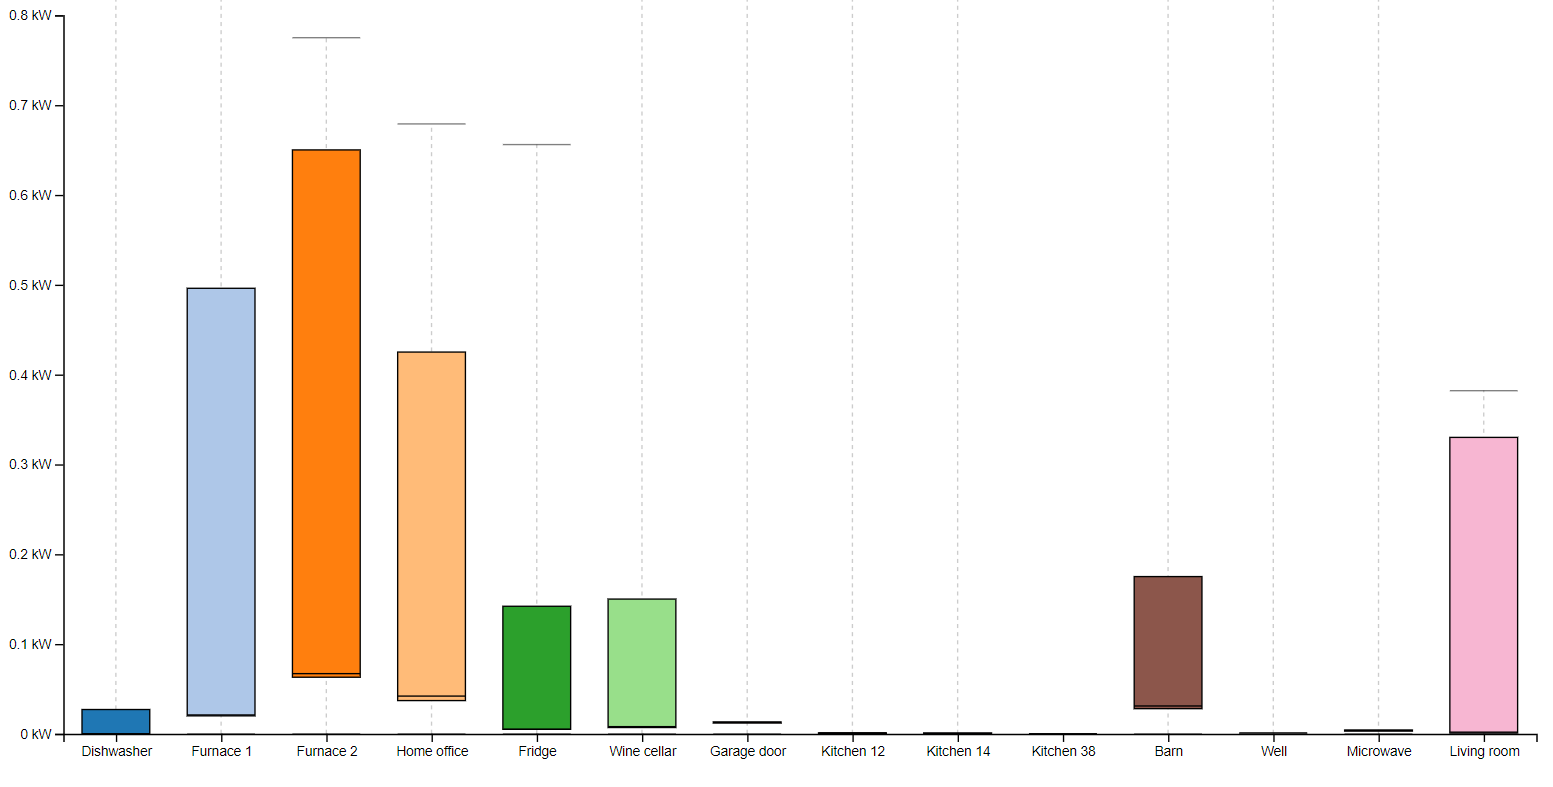
\includegraphics[width=\linewidth]{img/5.PNG} % Figure image
%	\caption{Box plot} % Figure caption
%\end{figure}

\documentclass[twoside,twocolumn]{article}

\usepackage{blindtext} % Package to generate dummy text throughout this template 

\usepackage[sc]{mathpazo} % Use the Palatino font
\usepackage[T1]{fontenc} % Use 8-bit encoding that has 256 glyphs
\linespread{1.05} % Line spacing - Palatino needs more space between lines
\usepackage{microtype} % Slightly tweak font spacing for aesthetics

\usepackage[english]{babel} % Language hyphenation and typographical rules
\usepackage{graphicx}
\usepackage[hmarginratio=1:1,top=32mm,columnsep=20pt]{geometry} % Document margins
\usepackage[hang, small,labelfont=bf,up,textfont=it,up]{caption} % Custom captions under/above floats in tables or figures
\usepackage{booktabs} % Horizontal rules in tables
\usepackage{subcaption} 

\usepackage{lettrine} % The lettrine is the first enlarged letter at the beginning of the text

\usepackage{enumitem} % Customized lists
\setlist[itemize]{noitemsep} % Make itemize lists more compact

\usepackage{abstract} % Allows abstract customization
\renewcommand{\abstractnamefont}{\normalfont\bfseries} % Set the "Abstract" text to bold
\renewcommand{\abstracttextfont}{\normalfont\small\itshape} % Set the abstract itself to small italic text

\usepackage{titlesec} % Allows customization of titles
\renewcommand\thesection{\Roman{section}} % Roman numerals for the sections
\renewcommand\thesubsection{\roman{subsection}} % roman numerals for subsections
\titleformat{\section}[block]{\large\scshape\centering}{\thesection.}{1em}{} % Change the look of the section titles
\titleformat{\subsection}[block]{\large}{\thesubsection.}{1em}{} % Change the look of the section titles

\usepackage{fancyhdr} % Headers and footers
\pagestyle{fancy} % All pages have headers and footers
\fancyhead{} % Blank out the default header
\fancyfoot{} % Blank out the default footer
\fancyhead[C]{Neural Network Project 2019/2020} % Custom header text
\fancyfoot[RO,LE]{\thepage} % Custom footer text

\usepackage{titling} % Customizing the title section

\usepackage{hyperref} % For hyperlinks in the PDF

%----------------------------------------------------------------------------------------
%	TITLE SECTION
%----------------------------------------------------------------------------------------

\setlength{\droptitle}{-4\baselineskip} % Move the title up

\pretitle{\begin{center}\Huge\bfseries} % Article title formatting
\posttitle{\end{center}} % Article title closing formatting
\title{DARTS: Deceiving Autonomous Cars with Toxic Signs} % Article title
\author{%
%\textsc{Fabio Montello (23124)  Leonardo Salvucci (1601997)}\thanks{A thank you or further information} \\[1ex] % Your name
\textsc{Antonino Di Maggio (1702628)  and Leonardo Salvucci (1601997)} \\[1ex] % Your name
\normalsize Sapienza - University of Rome \\ % Your institution
%\normalsize \href{mailto:john@smith.com}{john@smith.com} % Your email address
%\and % Uncomment if 2 authors are required, duplicate these 4 lines if more
%\textsc{Jane Smith}\thanks{Corresponding author} \\[1ex] % Second author's name
%\normalsize University of Utah \\ % Second author's institution
%\normalsize \href{mailto:jane@smith.com}{jane@smith.com} % Second author's email address
}
\date{\today} % Leave empty to omit a date
\renewcommand{\maketitlehookd}{%
\begin{abstract}
\noindent Recent studies show that the cutting edge deep neural networks are vulnerable to contradictory examples, deriving from small magnitude perturbations added to the input. With the advent of self-driving machines, the contradictory example, as we can imagine, can generate many complications: a car can interpret a signal incorrectly and generate an accident. In the following report, we want to analyze and test the problem, showing that it is possible to generate specific perturbations to the input images to confuse the model and, in some way, force the network prediction.
\end{abstract}
}

%----------------------------------------------------------------------------------------

\begin{document}

% Print the title
\maketitle

%----------------------------------------------------------------------------------------
%	ARTICLE CONTENTS
%----------------------------------------------------------------------------------------

\section{Introduction}

\lettrine[nindent=0em,lines=3]{I}n the following report we will explain our project in detail, aimed at explaining and implementing a good part of an existing project  described on the proposed paper \href{https://drive.google.com/open?id=1qBeGzMsa_wpiBdBe1HPRk_mxsomRyZY-}{DARTS: Deceiving Autonomous Cars with Toxic Signs}, written by Chawin Sitawarin, Arjun Nitin Bhagoji, Arsalan Mosenia, Prateek Mittal, from the  Princeton University, and Mung Chiang, from Purdue University.\\
\newline
The paper explained how to modify an existing traffic signal (or another generic signal), to deceive a model of an autonomous driving car.
In the paper various kind of attacks are presented:
\begin{itemize}
	\item \textbf{White box attack:} in this kind of attack, we have a trained model and its weights, so the aim is to create an adversarial image in order to mislead the specific model.
\newline
	\item \textbf{Black box attack:} in this case, we do not have a model, so the aim is to create an adversarial image that has to seems like another one for a generic model.
\end{itemize}
\newpage
The attacks mentioned can still be distinguished in:
\begin{itemize}
	\item \textbf{Targeted attack:} in this case, the aim is to choose a specific class of traffic signal such that the images (other signals, logos or custom signs) we are going to modify have to be recognized by the model as that.
\newline
	\item \textbf{Untargeted attack:} in this case the input image has to be a picture of a traffic sign and the aim is just to generate a wrong prediction, without specify a specific output class.
\end{itemize}

Or even:
\begin{itemize}
	\item \textbf{In-distribution attack:} the in-distribution attack consist in modify an image representing a traffic signal X, in order to seems like another traffic signal. It is called in-distribution because we have to modify an image that the model is trained to recognize in another image that the model knows. 
\newline
	\item \textbf{Out-of-distribution attack:} in this case the image is an image for which the model is not trained, in our case we have to cases of attacks:
        \begin{itemize}
          \item{\textbf{Logo attack:}} the image is a commercial logo (Burger King logo, KFC logo, etc.).
          \item{\textbf{Custom signs attack:}}  in this case we have an image representing a signal with no pattern, but just with plain color.
       \end{itemize}
\end{itemize}
We choose to implement the white box attack, for both the targeted and the untargeted attack and, for the targeted attack, both the in-distribution and out-of-distribution attacks.
For the untargeted attack, instead, we implemented only the in-distribution attack, because it would have no sense to implement the out-of-distribution attack.\\
\newline
We implemented two functions to perform two different kinds of attacks:
\begin{itemize}
	\item \textbf{Gradient attack};
	\item \textbf{Iterative attack}.
\end{itemize}
That we are going to present later in this report.


%------------------------------------------------

\section{The Dataset}

We use the \href{https://www.kaggle.com/meowmeowmeowmeowmeow/gtsrb-german-traffic-sign/data}{GTSRB - German Traffic Sign Recognition Benchmark} dataset. It is a multi-class, single-image classification challenge held at the International Joint Conference on Neural Networks (IJCNN) 2011.

\subsection{Structure}
The GTSRB has the following properties:
\begin{itemize}
	\item Single-image, multi-class classification problem;
	\item 43 classes;
	\item More than 50,000 images in total;
	\item Large, lifelike database;
	\item Reliable ground-truth data due to semi-automatic annotation;
	\item Physical traffic sign instances are unique within the dataset.
\end{itemize}

In the train sub-directory, there are 43 directories (numbered from 0 to 42), each of this directory represent a different kind of traffic signal, in this way:

\begin{center}
\begin{tabular}{ c c }
\textbf{ID} & \textbf{Traffic Sign Description} \\
0 & Speed limit (20km/h) \\
1 & Speed limit (30km/h) \\
2 & Speed limit (50km/h) \\
3 & Speed limit (60km/h) \\
4 & Speed limit (70km/h) \\
5 & Speed limit (80km/h) \\
6 & End of speed limit (80km/h) \\
7 & Speed limit (100km/h) \\
8 & Speed limit (120km/h) \\
9 & No passing \\
10 & No passing for vehicles over 3.5 metric tons \\
11 & Right-of-way at the next intersection \\
12 & Priority road \\
13 & Yield \\
14 & Stop \\
15 & No vehicles \\
16 & Vehicles over 3.5 metric tons prohibited \\
17 & No entry \\
18 & General caution \\
19 & Dangerous curve to the left \\
20 & Dangerous curve to the right \\
21 & Double curve \\
22 & Bumpy road \\
23 & Slippery road \\
24 & Road narrows on the right \\
25 & Road work \\
26 & Traffic signals \\
27 & Pedestrians \\
28 & Children crossing \\
29 & Bicycles crossing \\
30 & Beware of ice/snow \\
31 & Wild animals crossing \\
32 & End of all speed and passing limits \\
33 & Turn right ahead \\
34 & Turn left ahead \\
35 & Ahead only \\
36 & Go straight or right \\
37 & Go straight or left \\
38 & Keep right \\
39 & Keep left \\
40 & Roundabout mandatory \\
41 & End of no passing \\
42 & End of no passing by vehicles over 3.5 metric tons \\
\end{tabular}
\end{center}
\newpage
With the dataset, we even downloaded the images contained in the directory \textit{Original\char`_Traffic\char`_Signals\char`_samples}, which contains some samples in high definition, these are the images that we are going to modificate in order to be detected as other signals.
\newline
We even have to other directories:
\begin{itemize}
	\item Logo\char`_samples;
	\item Custom\char`_Sign\char`_samples.
\end{itemize}

\subsection{Data augmentation}
The dataset, originally, was highly unbalanced, as you can see in the following histogram:
\begin{figure}[!ht]
	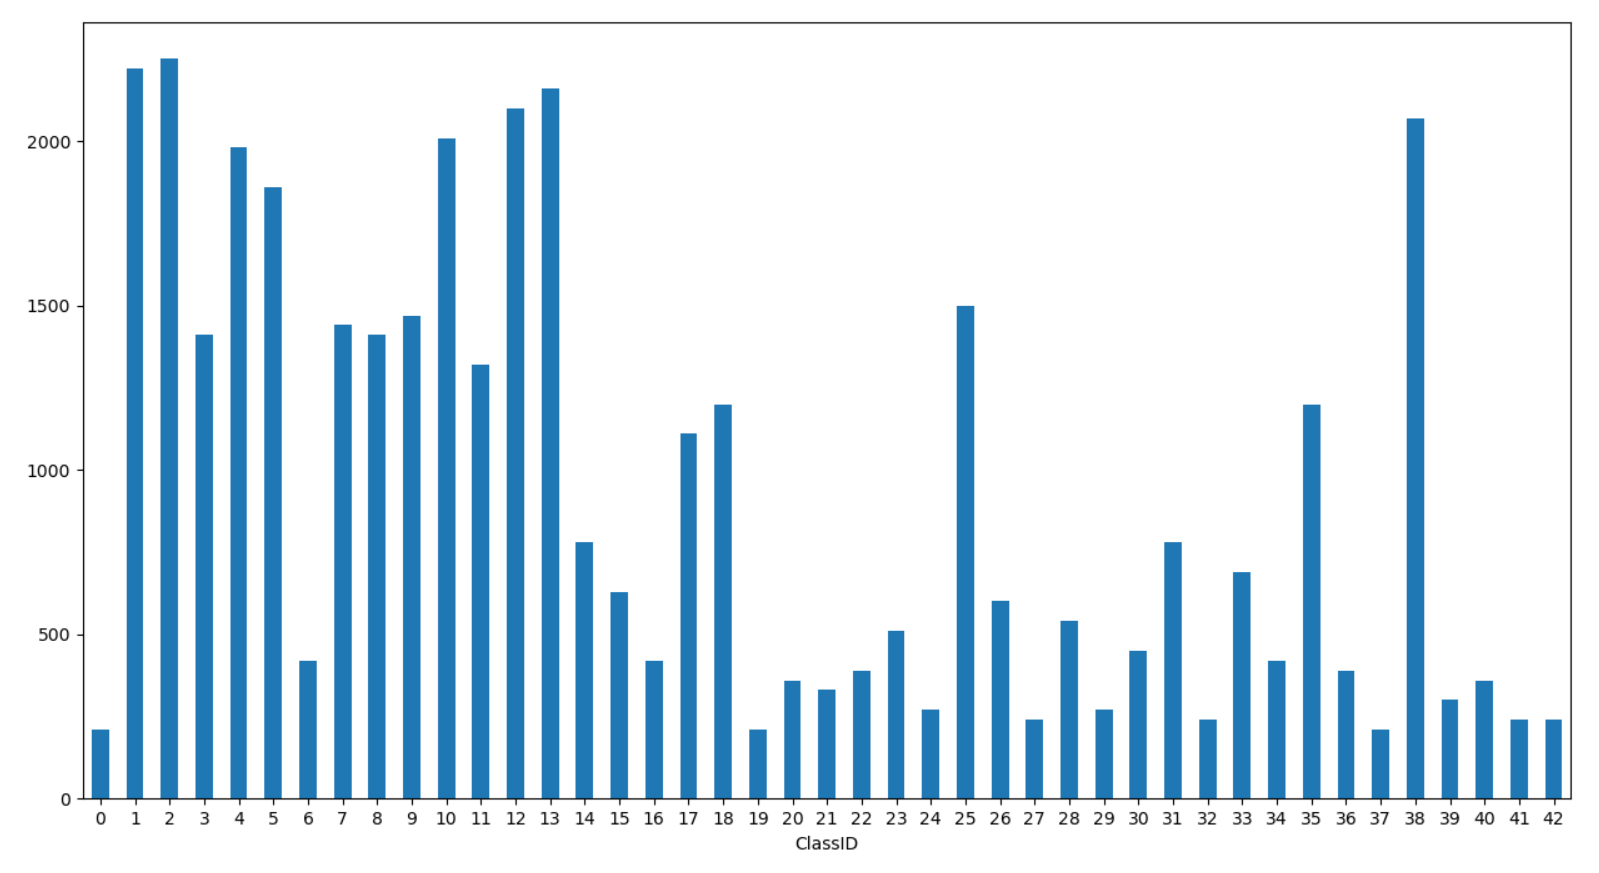
\includegraphics[width=\linewidth]{img/histo.PNG} % Figure image
	\caption{Dataset histogram} % Figure caption
\end{figure}

So, in order to obtain a better training, we had to balance it.
For this aim, we created the file called \textit{data\char`_augmentation.py}, containing four functions to apply a transformation to the existing images:
\begin{itemize}
\item \textbf{\textit{apply\char`_flip:}} in this function, we created two arrays to identify the signals that can be flipped, horizontally or vertically, without changing theirs meaning. Than, if a signal is flippable, we apply a flip of the image of the signal;
\begin{figure}[!ht]
\centering
\begin{subfigure}{.2\textwidth}
  \centering
  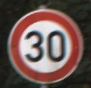
\includegraphics[width=.8\linewidth]{img/00001_00011_00027.png}
  \caption{Original}
  \label{fig:sub1}
\end{subfigure}%
\begin{subfigure}{.2\textwidth}
  \centering
  
\includegraphics[width=.8\linewidth]{img/1.png}
  \caption{Augmented}
  \label{fig:sub2}
\end{subfigure}
\end{figure}

\item \textbf{\textit{apply\char`_brightness:}} apply a random changing of the brightness of the signal;
\begin{figure}[!ht]
\centering
\begin{subfigure}{.2\textwidth}
  \centering
  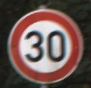
\includegraphics[width=.8\linewidth]{img/00001_00011_00027.png}
  \caption{Original}
  \label{fig:sub1}
\end{subfigure}%
\begin{subfigure}{.2\textwidth}
  \centering
  
\includegraphics[width=.8\linewidth]{img/2.png}
  \caption{Augmented}
  \label{fig:sub2}
\end{subfigure}
\end{figure}

\item \textbf{\textit{apply\char`_rotate\char`_image:}} apply a random rotation of the signal;
\begin{figure}[!ht]
\centering
\begin{subfigure}{.2\textwidth}
  \centering
  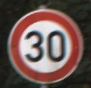
\includegraphics[width=.8\linewidth]{img/00001_00011_00027.png}
  \caption{Original}
  \label{fig:sub1}
\end{subfigure}%
\begin{subfigure}{.2\textwidth}
  \centering
  
\includegraphics[width=.8\linewidth]{img/3.png}
  \caption{Augmented}
  \label{fig:sub2}
\end{subfigure}
\end{figure}

\item \textbf{\textit{apply\char`_projection\char`_transform:}} apply a random perspective transformation of the signal;
\begin{figure}[!ht]
\centering
\begin{subfigure}{.2\textwidth}
  \centering
  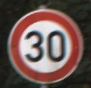
\includegraphics[width=.8\linewidth]{img/00001_00011_00027.png}
  \caption{Original}
  \label{fig:sub1}
\end{subfigure}%
\begin{subfigure}{.2\textwidth}
  \centering
  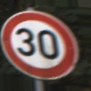
\includegraphics[width=.8\linewidth]{img/4.png}
  \caption{Augmented}
  \label{fig:sub2}
\end{subfigure}
\end{figure}
\end{itemize}
and these other to manage them:
\begin{itemize}
	\item \textbf{\textit{add\char`_data:}} if a class contains less than target size (target\_size = 2000) images, then one of the transformations is randomly applied to the original image and saved in the dataset;
	\item \textbf{\textit{rem\char`_data:}} otherwise, if a class contains more than target size images, we remove some of the existing images to balance the dataset classes;
\end{itemize}

Of course, the functions mentioned are only applied to the original images, to avoid increasing the images too many times and no longer being able to manage the changes. Then, the images are read, kept locally, and randomly modified until they reach the expected cardinality.
\newline
At this point, we obtained a balanced dataset, increasing it, from 51.839 to 80.000 images (2000 for each class). 
%------------------------------------------------

\section{The model}

\subsection{Model summary}
We implemented the withe box attack, so we needed a pre-structured and trained model to deceive, this is the summary of the model that we built:

%%% AGGIUNGERE SCREENSHOT DEL MODEL SUMMARY %%%

\begin{itemize}
	\item \textbf{Input layer:} We built an input layer to avoid to have to preprocess images that are too large, risking to saturate the memory of our computer, and even to have uniform images to give as input for our model. In order to do this, we passed to the model an \textit{INPUT\char`_SHAPE} = (32, 32, 3).
\newline
	\item \textbf{Convolutionary layers:} We used 3 convolutional layers, using 32 filters with 5x5 receptive field, to specify the strides of the convolution along the height and the width. This layers create a convolution kernel that is convolved with the layer input to produce a tensor of outputs. Each convolutional layer is followed by a \textit{ReLU} activation function.
\newline
	\item \textbf{Dropout layers:} This layers randomly sets a fraction rate of input units to 0 at each update during the training time, this is very useful to prevent overfitting. 
\newline
	\item \textbf{Pooling layers:} this layers help the model to remove un-useful informations, this is needed because, very often, neighboring elements contains very similar informations.
\end{itemize}

These three layers are repeated three times and then we insert a flatten layers for each pool of the previous layers, its aim is to change the shape from the 2D matrix produced by the previous layers into the correct shape to be interpreter by a dense layer. 
Than, before the dense layer, we merge the outputs of the three flatten layers.
At the end, just before the output, we have a dense layer, followed by another dropout layer and a last dense layer, that correspond to the output layer of our model.
\textbf{Optimizer:} as optimizer, we used the \textit{Adam}, with a learning rate equal to 0.0001.

\subsection{Training}
We trained the model with the augmented and balanced dataset, setting the number of epochs equals to 100. We checked if for 6 (patience=6) epochs the train accuracy do not improve, in that case, the training would be stopped.
\newline
The model reach very fast a very high accuracy for both train and validation, and indeed, at the epoch n.48, we obtained this following results:\\

\begin{tabular}{ |p{2cm}|p{2cm}|p{2cm}|p{2cm}|  }
 \hline
 \multicolumn{3}{|c|}{RESULTS} \\
 \hline
  & Train &Validation\\
 \hline
Accuracy&  0.9973    &0.9941\\
Loss&   0.0431  &  0.0632\\
 \hline
\end{tabular}

\subsection{Weights}
To avoid to re-train the model at every execution of the attacks, and even to charge every time the whole trained model, once we obtained the trained model, we saved its weights in a \textit{.hdf5} file named \textit{mltscl\_cnn.hdf5}.

\subsection{Model's test}

We tested the model on the test set proposed by the dataset. To execute it, as in the train, we used \href{https://keras.io/preprocessing/image/}{image data generator}, to process the images and pass them to the model for prediction.
We have achieved an excellent result reaching an accuracy of \textbf{96.41\%}. 

\section{Fast Gradient attack}
\subsection{Overview}
The \textbf{fast gradient attack} works by using the gradients of the neural network to create an adversarial example. For an input image, the method uses the gradients of the loss with respect to the input image to create a new image that maximises the loss. This new image is called the adversarial image.

\subsection{Untarget attack}
This method computes an adversarial image by adding a pixel-wide perturbation of magnitude in the direction of the gradient. This perturbation is computed with a single step, thus is very efficient in terms of computation time:
\[x_{adv} =  x + \varepsilon \cdot sign(\nabla x\quad J( \theta, x, y_{true}) \]
where:\\
- $x_adv$ : Adversarial image\\
- $x$: Original image\\
- $\varepsilon$: Small multiplier\\
- $y$: Original classification\\
- $\theta$: Model parameters\\
- $J$: Classification loss function\\

\subsection{Target attack}
In targeted attacks the attacker pretends to get the image classified as a specific target class, which is different from the true class. in this case in the direction of the negative gradient with respect to the target class:
\[x_{adv} =  x - \varepsilon \cdot sign(\nabla x\quad J( \theta, x, y_{target}) \]
where:\\
- $x_adv$ : Adversarial image\\
- $x$: Original image\\
- $\varepsilon$: Small multiplier\\
- $y$: Target class\\
- $\theta$: Model parameters\\
- $J$: Classification loss function\\

\subsection{Execution}
To execute the attack we have implemented the following function:
\newline
\[ fg(model, x, y, mask, target)\]
where:\\
- $model$ : The trained model to attack\\
- $x$: A numpy array containing the samples to attack.\\
- $target$: True if it's a TARGET attack, False otherwise\\
- $y$: A numpy array containing the respective labels. It is important to note that if it's target attack the list contains always the same value (Target class), otherwise it contains, for each cell, the respective label. \\
- $masks$: The list of respective masks to restrict gradient update only on the image’s portion that contain the signal, excluding the background (Optional).\\
\newline
The function returns a numpy array containing the adversarial images that we save in a specific folder.

\subsection{Attack's description}
First of all, we initialize the variable \textit{x\char`_adv}, that will contains our adversarial example, as a numpy array of zeros that as the same dimension of our input images plus the length of the magnitude list. Than we have to create a function that have to calculate the gradient of an input image, with respect of the Keras model. In order to do this we created a function called \textit{gradient\char`_fn}, that takes as input the model and return the gradient, using the gradient function provided by the \textit{keras.backend} library and return the function the we need.\\
\newline
In order to perform the attack, we have to iterate through the input images in \textit{x} and, for each image, we have to calculate its gradient using the function \textit{grad\char`_fn} that we created. Than we applicate the mask and normalize the gradient.
\newline
At the end, we create the perturbation according to a specific value and it returns the adversarial images clipped according the function \textit{numpy.clip} with interval [0, 1], in this case, in the \textit{x\char`_adv} array, the values smaller that 0 are converted to 0, and the ones bigger than 1 are converted to 1.


\section{iterative attack}
The \textbf{iterative attack} is more sophisticated in confront of the fast gradient one. It moves a benign sample in the gradient direction one small step at a time for n steps.

\subsection{Execution}

The main function to perform this attack is defined in this way:
\[ iterative(model, x, y, mask, target) \]
where:\\
- $model$ : The trained model to attack\\
- $x$: A numpy array containing the samples to attack.\\
- $target$: True if it's a TARGET attack, False otherwise\\
- $y$: A numpy array containing the respective labels. It is important to note that if it's target attack the list contains always the same value (Target class), otherwise it contains, for each cell, the respective label. \\
- $masks$: The list of respective masks to restrict gradient update only on the image’s portion that contain the signal, excluding the background (Optional).\\
\newline
The function returns a numpy array containing the adversarial images that we save in a specific folder.

\subsection{Attack's description}
The first part of this attack is very similar to the fast gradient attack, indeed: First of all, we initialize the variable \textit{x\char`_adv}, that will contains our adversarial example, as a \textit{numpy} array of zeros that as the same dimension of our input images plus the length of the magnitude list.\\
\newline
Than we have to create a function that have to calculate the gradient of an input image, with respect of the Keras model. In order to do this we created a function called gradient\char`_fn, that takes as input the model and return the gradient, using the gradient function provided by the \textit{keras.backend} library and return the function the we need. In order to perform the attack, we have to iterate through the input images in x and apply the mask.
But, at this point, we have to iterate again according to the number of steps we set (we set 40 steps).

\subsection{Observations}
First attack have lower success rates when compared to the iterative methods in white box attacks, however when it comes to black box attacks the basic single-shot methods turn out to be more effective. The most likely explanation for this is that the iterative methods tend to overfit to a particular model.

\section{Attack settings}
Before starting the attacks, we had to set some constants, in order to perform and store results correctly.

\subsection{Variables' setting}
It is important to find a good values for the magnitude such that the image can be modified nor too less (it would be very difficult to mislead the model), nor too much (it would be obvious, even for a human, that a sign is not the original one).\\
\newline
Then we create another variabile, called \textit{attack\char`_type}, we can assign to this variable three possibile values:
\begin{itemize}
	\item \textbf{\textit{IN\char`_DISTRIBUTION:}} if we want to perform the in-distribution attack. In this case, if we are performing a targeted attack, we delete from the input samples the images having as label the target;
	\item \textbf{\textit{LOGO:}} if we want to perform the logo attack;
	\item \textbf{\textit{BLANK:}} if we want to perform the custom signs attack.
\end{itemize}

Than, if we want to perform the targeted attack, we can create a variable \textit{tg} that must contain the label of the target class.

At this point we load our samples, the masks, in the \textit{x\char`_smp} and masks variables using the \textit{load\char`_samples} function, the path of the directory of the images will change according to the value of \textit{attack\char`_type}.

\section{Attacks evaluation}
To evaluate our attacks, we created two pandas data frames (one for the evaluation of the fast gradient attack and the other for the evaluation of the iterative attack), with the following columns:
\begin{itemize}
	\item \textbf{path\char`_original:} the path of the original image;
	\item \textbf{prevision\char`_original:} the prevision of the original image made by the model;
	\item \textbf{path\char`_adversarial:} the path of the adversarial image created by the attack;
	\item \textbf{prevision\char`_adv:} the prevision of the adversarial image made by the model;
	\item \textbf{success:} we have two cases:
	\begin{itemize}
		\item \textbf{Untargeted attack:} 
		\begin{itemize}
			\item 1, if prevision\char`_adv $\neq$ prevision\char`_original;
			\item 0, otherwise.
		\end{itemize}
		\item \textbf{Targeted attack:}
		\begin{itemize}
			\item 1, if prevision\char`_adv = target;
			\item 0, otherwise.
		\end{itemize}
	\end{itemize}
\end{itemize}

At this point, each type of attack has its own folder to save its images and its own\textit{.CSV} file, and the opened and read to compute the accuracy of the two attacks.


\section{Detection phase}
The detection phase is very important, since the network must classify images of the real world, with backgrounds, etc. So, this phase allows you to detect the area of interest for the model of the image, in our case a circle, clean it and send it to the model to classify it.
\begin{figure}[!ht]
	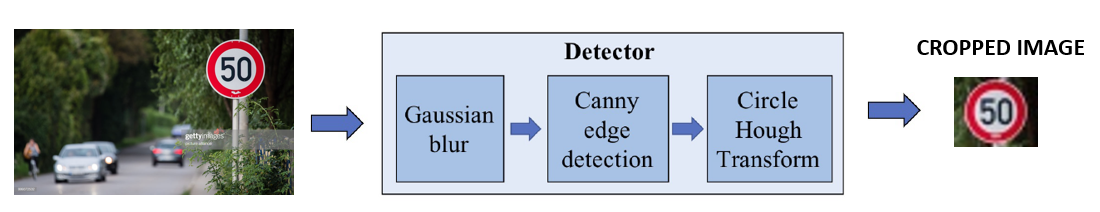
\includegraphics[width=\linewidth]{img/6.PNG} % Figure image
	\caption{Datection phase} % Figure caption
\end{figure}

This phase is characterized by five functions, starting from the original image:\\
\newline
\textbf{Gaussian Blur}: This technique (Image Smoothing) help in reducing the noise. Any sharp edges in images are smoothed while minimizing too much blurring.\\
\newline
\textbf{Gray Scale}: This technique convert it to gray scale.\\
\newline
\textbf{Canny Edge detection}: This technique allows to easily detect the edges, distinguishing them in more or less relevant.\\
\newline
\textbf{Circle Hough transform}: is an image transform that allows for circular objects to be extracted from an image, even if the circle is incomplete. The transform effectively searches for objects with a high degree of radial symmetry, with each degree of symmetry receiving one "vote" in the search space. we specify the expected radius of interest and the quantity of circles to detect (in our case one). We set the \textit{mg\char`_ration} parameter to 0.4, to retrieve just the portion of the signal and to do take as less background as possible, and \textit{n\char`_circle} to 1, to look for exactly one circle (otherwise, it could find even the image portions that could be identified as circle, but with lower probability, incrementing the probability to have errors).

\section{Real time detection}

In our project we have also implemented a phase of detection and classification in real time. In our test, for simplicity, we used the webcam of our pc, showing images of some road signs. The sign is detected in the camera frame and then classified by our model, showing the relative label above the frame that identifies the road sign.\\
\newline
We show an example in the following image:
\begin{figure}[!ht]
	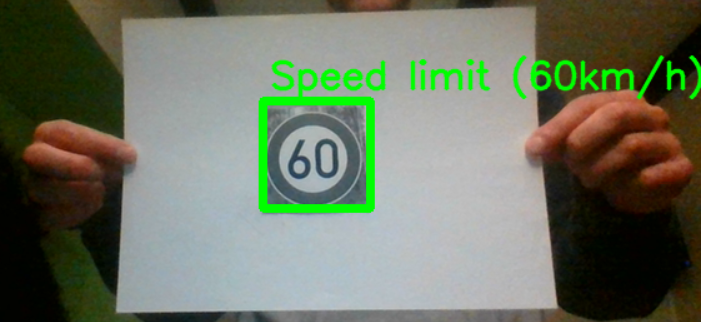
\includegraphics[width=\linewidth]{img/real.PNG} % Figure image
	\caption{Real time analysis} % Figure caption
\end{figure}

Intuitively, this process can be generalized to other applications, for example, by mounting the camera in the dashboard of our car.

%------------------------------------------------


%Than we perform the attacks:
%\begin{itemize}
%	\item If we are performing an in-distribution attack we can choose to do a targeted or an untargeted attack;
%	\item If we performing an out-of-distribution attack (logo or custom signs), we can only do a targeted attack, because the model is not trained for the input images.
%\end{itemize}

%We perform both the fast gradient and the iterative attack, and we save the outputs in the variables \textit{x\char`_fg} and \textit{x\char`_it}.

%------------------------------------------------



\section{Result}

We tested all kinds of attacks and, using as target class: 
%INSERIRE NUMERO E DESCRIZIONE CLASSE TARGET%
 we obtaining the following results (in \% of accuracy):
 \newline
 
 \begin{itemize}
 	\item \textbf{In-distribution attack:}
 	\begin{itemize}
 		\item Fast gradient attack:
		\begin{itemize}
			\item Targeted:
			\item Untargeted: 
		\end{itemize}
		\item Iterative attack:
		\begin{itemize}
			\item Targeted:
			\item Untargeted:
		\end{itemize}
	\end{itemize}
	
	\item \textbf{Logo attack:}
	 	\begin{itemize}
 		\item Fast gradient attack:
		\begin{itemize}
			\item Targeted:
		\end{itemize}
		\item Iterative attack:
		\begin{itemize}
			\item Targeted:
		\end{itemize}
	\end{itemize}
	
	\item \textbf{Custom Signs attack:}
	 	\begin{itemize}
 		\item Fast gradient attack:
		\begin{itemize}
			\item Targeted:
		\end{itemize}
		\item Iterative attack:
		\begin{itemize}
			\item Targeted:
		\end{itemize}
	\end{itemize}
\end{itemize}

%------------------------------------------------


\section{Conclusions}

\section*{Useful links}
\begin{itemize}
\item \textbf{GitLab directory:}\\
\url{github.com/leonardouniromasalvucci/DARTS-Deceiving-Autonomous-Cars-with-Toxic-Signs-}\\

\item \textbf{Link to download the model:}\\
\url{kaggle.com/meowmeowmeowmeowmeow/gtsrb-german-traffic-sign/data}\\

\item \textbf{Link to download the dataset:}\\
\url{drive.google.com/open?id=1wHJzXTC__lVbN86NPu_hUpoaSxM9-v5m}\\

\item \textbf{Link to the original paper:}\\
\url{arxiv.org/pdf/1802.06430.pdf}\\
\end{itemize}

\section*{Contacts}
\begin{itemize}
\item \textbf{Antonino Di Maggio's LinkedIn profile:}\\
\url{linkedin.com/in/antonino-di-maggio/}\\

\item \textbf{Leonardo Salvucci's LinkedIn profile:}\\
\url{linkedin.com/in/leonardo-salvucci/}\\
\end{itemize}
%----------------------------------------------------------------------------------------
%	REFERENCE LIST
%----------------------------------------------------------------------------------------

%\begin{thebibliography}{99} % Bibliography - this is intentionally simple in this template

%\bibitem[Figueredo and Wolf, 2009]{Figueredo:2009dg}
%Figueredo, A.~J. and Wolf, P. S.~A. (2009).
%\newblock Assortative pairing and life history strategy - a cross-cultural
%  study.
%\newblock {\em Human Nature}, 20:317--330.
 
%\end{thebibliography}

%----------------------------------------------------------------------------------------

\end{document}
